\begin{figure}[H]
\centering
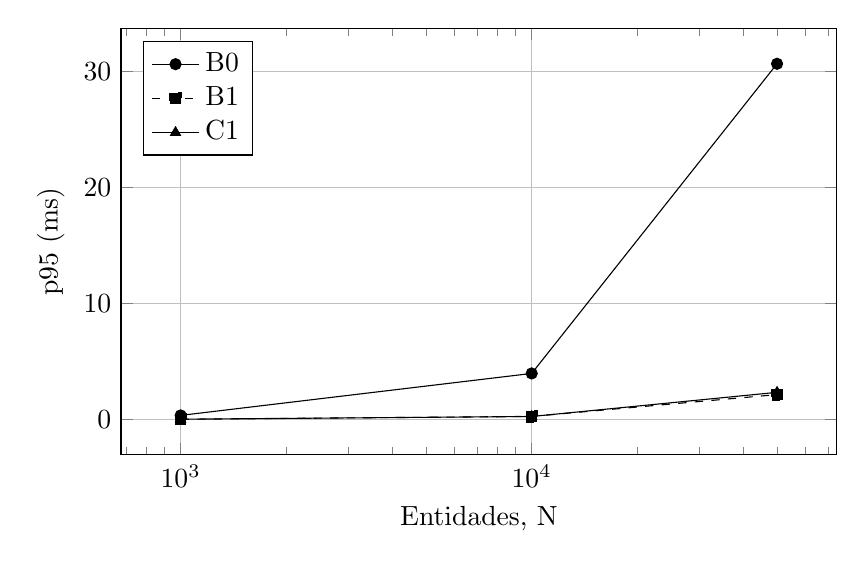
\begin{tikzpicture}
\begin{axis}[width=.88\textwidth,height=7cm,grid=major,legend pos=north west,
xlabel={Entidades, N},ylabel={p95 (ms)},xmode=log,log basis x=10]
\addplot[black,mark=*,solid] coordinates {(1000,0.37318505) (10000,3.9848564) (50000,30.635296)};
\addlegendentry{B0}
\addplot[black,mark=square*,dashed] coordinates {(1000,0.0363792) (10000,0.2859542) (50000,2.1637087)};
\addlegendentry{B1}
\addplot[black,mark=triangle*,solid] coordinates {(1000,0.04605815) (10000,0.27909345) (50000,2.3594251)};
\addlegendentry{C1}
\end{axis}
\end{tikzpicture}
\caption{Latencia p95 de P1 para el perfil R.}
\end{figure}